\documentclass[../main.tex]{subfiles}

\begin{document}

\section{Electrolytes}
\label{sec:electrolytes}
\subsection{Introduction (Arihant)}% and historical context}
\label{sec:introduction_electrolytes}
Some of the important challenges for development of Li-ion rechargeable batteries for electric vehicles are development of a non-flammable safe electrolyte with large operating voltage window that can develop rapidly a SEI layer to prevent plating of Li on a carbon anode and allows fast charging of the battery.\cite{Goodenough2010} Figure \ref{fig:electrolyte} schematically shows the electronic energy levels in electrode and electrolyte of a battery cell. If the anode electrochemical potential, $\mu_{A}$ is above the lowest unoccupied molecular orbital (LUMO) of the electrolyte, the electrolyte will get reduced, unless a passivating layer creates an energy barrier for transfer of electrons from the anode to the electrolyte LUMO. Similarly, if the cathode electrochemical potential $\mu_{C}$ is below the highest occupied molecular orbital (HOMO) of the electrolyte, the electrolyte will get oxidized, unless a passivating layer creates an energy barrier for transfer of electrons from the electrolyte HOMO to the cathode. Therefore, the electrochemical potentials $\mu_{A}$ and $\mu_{C}$ should lie within the the energy separation (E$_g$) between the LUMO and the HOMO of the electrolyte, which constrains the open-circuit voltage $V_{\rm oc}$ of a battery cell:

\begin{equation}
    eV_{\rm oc}=\mu_{A}-\mu_{C}\leq E_{g}
\end{equation}

where $e$ is the magnitude of the electron charge. %A passivating SEI layer at the electrode/electrolyte boundary can give a kinetic stability to a larger $V_{\rm oc}$ provided that $eV_{\rm oc}-E_{g}$ is small. 
The formation of the passivating SEI layer comes with the cost of irreversible capacity loss.

\begin{figure}
    \centering
    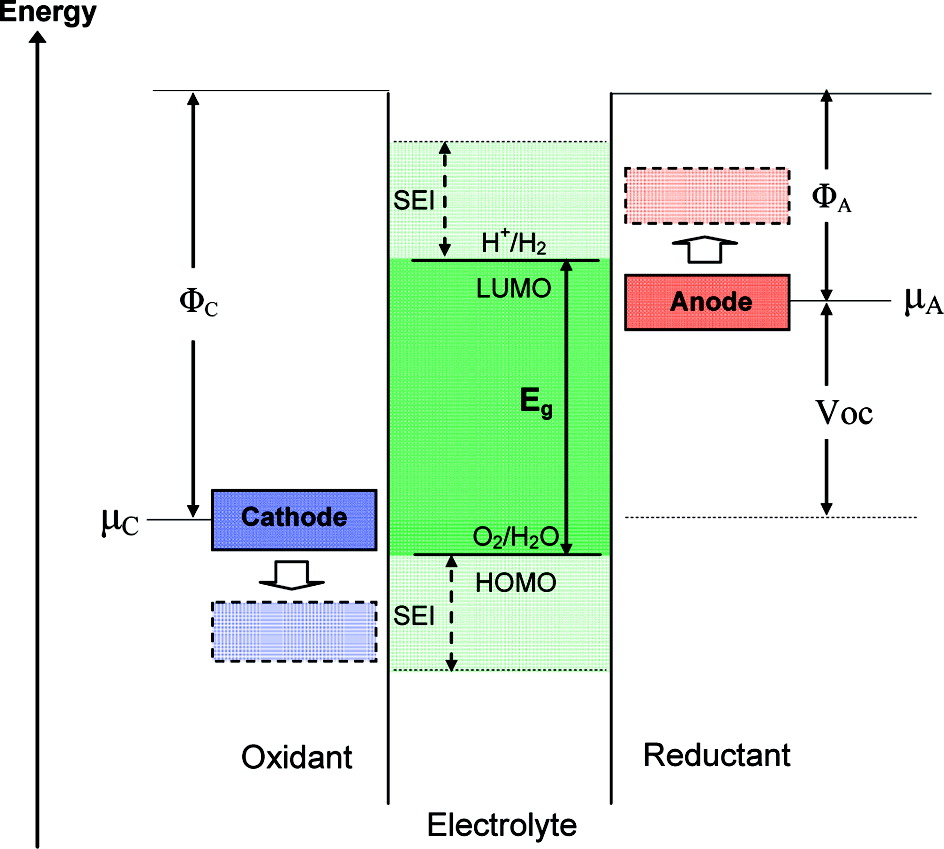
\includegraphics{figures/electrolyte.jpeg}
    \caption{Schematic open-circuit energy diagram of an aqueous electrolyte. $\Phi_{A}$ and $\Phi_{C}$ are the anode and cathode work functions. $E_{g}$ is the window of the electrolyte for thermodynamic stability. A $\mu_{A}>$ LUMO and/or a $\mu_{C}<$ HOMO requires a kinetic stability by the formation of SEI layer. Reproduced from Ref. \citenum{Goodenough2010} }
    \label{fig:electrolyte}
\end{figure}

The gap $E_g$ for an aqueous electrolyte is $ \approx 1.3 $  eV which severely limits the open circcuit voltage $V_{oc}$. In order to obtain a higher open circuit voltage $V_{oc}$, non-aqueous electrolytes with larger $E_g$ seem promising candidates. Several lithium salts are soluble in some non-aqueous solvents and polymers, which has led to the development of modern Li-ion batteries.

Apart from larger thermodynamic stability window, another requirement is high ionic conductivity ($>10^{-4}$ S/cm) in the electrolyte and across the electrode-electrolyte interface for a high rate-capability. Figure \ref{fig:conductivity} shows the ionic conductivities of common non-aqueous  electrolytes.\cite{Kamaya2011} These can be broadly classified into liquid and solid electrolytes. In the next subsections, we describe some of the liquid and solid electrolytes, their ionic diffusivity and stability. 

\begin{figure}[htbp]
    \centering
    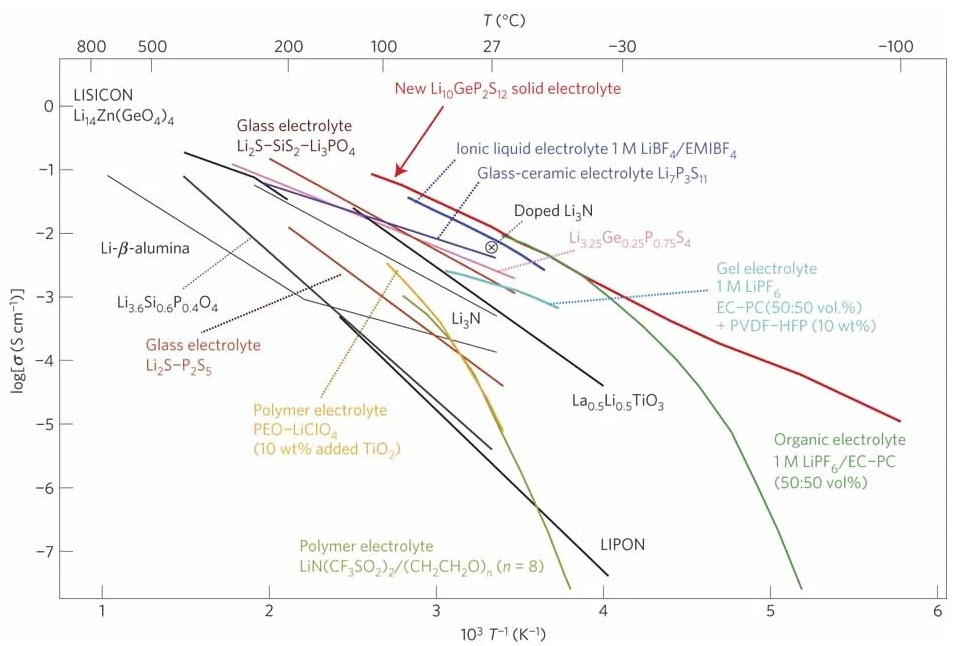
\includegraphics[scale=0.6]{figures/conductivity.jpg}
    \caption{Ionic conductivity of different electrolytes, reproduced with permissions from Ref. \citenum{Kamaya2011}}
    \label{fig:conductivity}
\end{figure}

%General picture and types of electrolytes. The importance of moving from liquid to solids and the challenges involved.
%General description, broad picture.
%Compatibility between electrolyte types and anode/cathode types. In terms of the cathodes, we discuss layered oxides (NMC), layered oxides (LiMn$_2$O$_4$), and polyanions (LiFePO$_4$), so if we can link electrolytes to these specific materials, it would prelude to the cathodes section. Similarly to the anodes section if possible?




\subsection{Liquid Electrolytes (Sam/Arihant)}
\label{sec:Liquid_electrolytes}
% \subsubsection{Introduction (MZ/Arihant)}
%Brief intro to liquid electrolytes, highlighting the importance of atomistic modelling. Introducing widely used liquid electrolytes, mixtures with solvents/common solvents. What materials/properties will be discussed here i.e. used as examples.

%Maybe something about impotance of electrolytes, like:
%Understanding electrolytes is very important in overall electric batteries modeling, as electrolytes may be "bottle-necks" in carrying high current density. may strongly affect degradation mechanisms, thermal effects, etc.

% The most widely used liquid electrolyte in Li-ion batteries is LiPF$_6$ in a solvent, which is typically a mix of two or more solvents, for example propylene carbonate (PC), ethylene carbonate (EC), ethyl methyl carbonate (EMC), dimethyl carbonate (DMC), in order to achieve competing objectives such as ability to dissolve high concentration of salt, low viscosity, high dielectric constant, at typical operational temperatures. Cyclic carbonates (EC, PC) have higher dielectric constant but also high viscosity, while ``linear'' carbonates (DMC, EMC) low viscosity but also low dielectric constant; for that reason often mixtures of solvents are used to optimise performance in a specific application are used.

% \begin{figure}
%     \centering
%     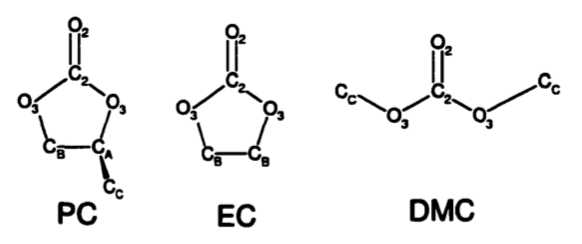
\includegraphics[scale=0.3]{figures/LE1.PNG}
%     \caption{Molecular structure for solvents: propylene carbonate (PC), ethylene carbonate (EC), dimethyl carbonate (DMC).}
%     \label{fig:LE1}
% \end{figure}

\subsubsection{An introduction to modelling liquid electrolytes}
The modelling of the liquid electrolytes for conventional batteries is a broad and diverse field. Over the past 20-30 years atomistic modelling has helped shape the fundamental physics of liquids, determining new physical basis and validating decades old pen and paper theories of concentrated electrolytes.The development of liquid electrolytes can presented from an applications approach or a methods approach. Here, we focus on the development of liquid electrolyte models and the considerations needed when modelling these materials.

Atomistic modelling of liquid electrolytes can be broadly separated into \textit{ab-initio} and classical molecular dynamics (MD) modelling (c.f. section~\ref{sec:molecular_dynamics}). These techniques are complementry and can be used to aid the other. For example, first principles calculations are able to provide information on the electron distribution which are required for paramatersing the non-bonded components force fields used in classical MD.
Classical MD can also be used to provide the starting conditions for DFT calculations. At their point of highest symbiosis \textit{ab-initio} and classical methods are combined in quantum mechanics/molecular mechanics (QM/MM) studies, where the larger system is treated classically with a smaller sub region being modelled using \textit{ab-initio} methods.

In this section we will first discuss the separate use of both \textit{ab-initio} and classical MD methods, as applied to the liquid electrolyte bulk. Following this we will discussion solid--electrolyte interface (SEI) from the perspective of the liquid electrolyte (complementary to the solid focused SEI discussion given in section~\ref{sec:SEI}).

\subsubsection{\textit{ab-initio} modelling of liquid electrolytes}
\textit{Ab-initio} modelling using DFT (c.f. section~\ref{sec:dft}) provides a wide variety functionals, each with different levels of described physics. A major limitation of this approach is the feasible time and length scales reachable due to high computational cost; generally restricting to a maximum of 3 nm $\times$ 3 nm $\times$ 3 nm and tens to hundreds of pico-seconds. The limited time and length scales both introduce inaccuracies and irregularities in the calculations. Small length scales (box size) introduce issues regarding long to medium range correlations of atoms and molecules. As liquid do not exhibit long range order, the presence of periodic images that are located at exactly a cell width in all direction introduces an unphysical correlation. This is observed in the modelling of systematically disordered solids in smaller cells. Beyond truncating the radial distribution function (RDF) to a shorter distant (i.e. half the shortest distance between periodic images) than is optimal, this effect will also introduce (normally small) inaccuracies in thermodynamic and dynamic quantities\cite{Binder2009book, yeh_system-size_2004,botan_diffusion_2015,horbach_finite_1996}. These inaccuracies are of a particular concern in liquid electrolytes as the electrostatic interactions between ions gives rise to longer range interactions \cite{coles_correlation_2020}. Use of a relatively short Debye length of concentrated electrolytes to counteract any correlations with periodic images is not plausible as the Debye H\"{u}ckel screening length is not relevant in these systems. This is because charge oscillatory screening with a decay length on the same order of magnitude as the standard box length is observed in these systems\cite{coles_correlation_2020}. The short time scale of \textit{ab-initio} simulations can, particularly for more viscous liquids, lead to highly non-ergodic (fully-sampled) simulations. When snapshots throughout the whole trajectory are highly correlated\cite{frenkel_understanding_2002}, this can lead to problems for both dynamic and equilibrium studies. 

Neither the issue of time correlation or finite size effects has a significant detrimental to the results of \textit{ab-initio} studies. However, in specific studies where they need to be avoided, or where a quantum description of a liquid electrolyte provides no significant advantage over a classical description, it is beneficial to turn towards far less computationally expensive (and thus larger and longer) classical simulations.

\subsubsection{Classical modelling of liquid electrolytes}
Classical simulations of liquid electrolytes includes force fields based molecular dynamics (c.f. section~\ref{sec:molecular_dynamics}) and the related field of classical Monte Carlo (c.f. section~\ref{sec:monte_carlo}). % before moving to discuss their implementation and analysis.
% \subsubsection{Classical force fields for liquid electrolytes}
Classical molecular dynamics is a broad field which uses many different types of force fields for different studies. The development of force fields for ionic solids is described in section~\ref{sec:potential_fitting}, whereas here we evaluate the force fields used for liquid electrolytes and the considerations need to develop them. The focus here will be placed on the development of force fields for ionic liquid electrolytes, however, similar processes have taken place for organic solvents, which we will link to throughout the discussion.

Electrolyte solvents from water, to molecular solvents and ionic liquids, pose a challenge that is not normally present in the solid state, specifically the need to model covalent bonding. This is achieved by splitting the potential acting on each atom into bonding and non-bonding contributions. The non-bonding component accounts for the effects of electrostatics, dispersion, and degeneracy pressure; and the bonding component accounts for the effects covalent bonding. In classical modelling of liquid electrolytes we are mainly interested in the behaviour within the electrolyte's electrochemical window, therefore, the vast majority of classical studies model bonds with unbreakable, harmonic, potentials. There are four distinct types of bonded potential \cite{lindahl_gromacs_2021, frenkel_understanding_2002}: bonds, angles, dihedrals, and improper dihedrals. These can be traced back to the parameterisation of force fields, such as OPLSA-AA\cite{canongia_lopes_clp_2012,jorgensen_development_1996}, and are often parameterised from spectroscopic force constants. There are many ways of defining boned potential types, as described in the manuals of the popular Gromacs\cite{lindahl_gromacs_2021} and Lammps\cite{PLIMPTON19951} software, though this discussion is beyond the scope of this review. Atoms which are subject to a bonded potential are often wholly, or in the case of dihedrals in OPLS-AA, partially excluded from non-bonded interactions as part of a force fields design. In larger molecules, intramolecular interactions beyond these exclusions will often play an important role in the description of a molecule.

Bonds can also be represented using Constraints, through algorithms such as LINCS\cite{hess_lincs_1997}, SHAKE\cite{ryckaert_numerical_1977}, and RATTLE\cite{andersen_rattle_1983}. These convert a molecule to a rigid body with fixed equilibrium bond lengths (or angles). This method gives greater computational efficiency by decreasing the degrees of freedom and allows for an initial simulation with an undefined force field. It should be noted that while constraining a C-H bond may have little effect, constraining other bonds or angles could readily affect structural and dynamic properties \cite{de_wijn_internal_2011, hess_lincs_1997}, and a constrained molecule is a single (non-spherical) statistical mechanical unit.

When developing force fields, generally, it is the non-bonded force field components, in particular the partial charges on atoms, which are more frequently varied. A common model for liquids electrolytes is the OPLS-AA force field developed by \citeauthor{jorgensen_development_1996} \cite{jorgensen_development_1996}. The non-bonded force field components consist of a Lennard-Jones potential, modelling the repulsive degeneracy pressure and the attractive dispersion, and a coulombic term, solved via Ewald summation \cite{ewald_berechnung_1921} or Ewald based grid method \cite{darden_particle_1993,deserno_how_1998,yeh_ewald_1999}.

The Canongia Lopes \& Padua (CP\&P) force field \cite{canongia_lopes_clp_2012, canongia_lopes_modeling_2004, canongia_lopes_molecular_2004, canongia_lopes_molecular_2006} was created to describe a wide range of ionic liquid cations and anions. It was originally based on the OPLS-AA force field for organic molecules (used for organic solvents in electrolytes), with non-bonded potentials and partial charges varied to model the ionic components. The charges on the individual molecules are obtained form first principles calculations (DFT), in this case by use of the charge mapping algorithm CHelpG\cite{canongia_lopes_clp_2012} (though other algorithms may also be used\cite{spackman_potential_1996,breneman_determining_1990,singh_approach_1984}). At the core of its design CL\&P had the principle of miscibility, meaning there is a separate force field for each cation and anion, with no change implemented for an ion on the basis of its counter-ion.

CL\&P and OPLS-AA based force fields for ionic liquid and molecular lithium salt solutions are often employed with charge rescaling, equivalent to adjusting to relative permittivity of the media to a value other than one. The rescaling decreases the charge on ions and resolves the problem of OPLS-AA based force fields giving high viscosity for concentrated electrolytes, ionic liquids and their mixtures\cite{schroder_comparing_2012, schroder_polarizable_2020, shimizu_structural_2015}. Charge rescaling accounts for the effect of polarisability on the strength of electrostatic interactions between ions. However, other force fields have been defined to account directly for polarisability \cite{schroder_polarizable_2020}.

As described in section~\ref{sec:potential_fitting}, polarisability can be introduced to a force field using a type of core-shell model, also called the Drude oscillator model \cite{schroder_polarizable_2020, schroder_comparing_2012, lindahl_gromacs_2021}. The Drude oscillator model is computationally cheap and is core to the polarisable ionic liquid force field developed from CL\&P by \citeauthor{schroder_comparing_2012} \cite{schroder_comparing_2012}. A more advanced representation of polarisability can be provided by an intrinsically polarisable force fields, normally based on the Fumi-Tosi potential. Polarisability is incorporated within the non-bonded functional form of the non-bonded terms which give an intrinsic polarisability \cite{madden_covalent_1996, borodin_polarizable_2009, schroder_polarizable_2020, borodin_litfsi_2006,bedrov_molecular_2019,bedrov_influence_2010}. This provides the best description of polarisability in a classical force field, however, there is an associated higher computational cost. These force fields are also not available in many of the major molecular dynamics codes, and will often require a special code in order to be run (such as the metalwalls \cite{marin-lafleche_metalwalls_2020}).

The development of force fields for metal cations has seen an equal level of discussion and interest. When considering cations, such as Lithium or Magnesium\cite{mamatkulov_force_2013,mamatkulov_force_2018}, modelling these ions as small mildly dispersive impolarisable spheres is a rather uncontroversial choice (provided we are working in conditions where there is no chance of ionisation)\cite{schroder_polarizable_2020}. In order to maintain compatibility with solvent force fields such as OPLS-AA and the simple point charge (SPC) water molecules these ions are frequently modeled as Lennard Jones spheres. In the Lennard Jones force fields of alkali and alkali earth metal cations a wide range of values of $\sigma$ (excluded volume) and $\epsilon$ (interaction strength) are used. This is because the basic energetics associated with one of these force fields can be recovered for many sigma values provided they are paired with a corresponding and correct epsilon value. The specific decision depends on the exact sort of properties that need to be accurately reproduced, such as the location and height of certain peaks within an RDF and the activity of solutions in a more concentrated regime\cite{mamatkulov_force_2013}. It is worth noting that many force fields used to modeled the electrolytes of specific interest to us here, were parameterised for aqueous solutions.

\subsubsection{MD and analysis of liquid electrolytes}
%Here, we discuss the specific methods applied to model and analyse liquid electrolytes. In this section we will touch on some specific analyses and methods of particular utility to this specific field\footnote{A reader with more general interest is directed towards Frenkel and Schmit\cite{frenkel_understanding_2002}, while a reader with a specific interest in the physics of electrolyte solutions is directed toward Chapter 5 of Hansen and McDonnald}.

%Diffusion
Diffusion (c.f. section~\ref{sec:diffusion}) plays a critical role in the operation of liquid electrolytes through its impact on conductivity. However, in liquid electrolytes its impact goes deeper as the dielectric constant of liquids consists of both dipolar and ionic contributions. These two contributions can be obtained by analysis of the dipole orientation and current auto-correlation functions using the Einstein-Helfand method. For example, \citeauthor{coles_correlation_2020} performed this analysis on four liquid electrolytes (three in aqueous solvent and one in a common organic solvent mixture): aqueous solutions of LiCl, NaI, and LiTFSI, as well as the same LiTFSI salt solvated in an equimolar mixture of DME and DOL \cite{coles_correlation_2020}. Here, it was shown that for polar solvents the dipolar contribution is nearly always dominant, with current acting as correction which could feasibly be neglected (particularly for more dilute systems). For ionic liquids, such as 1-ethyl-3-methyl-imidazolium dicyanoamide (EMIM$^+$), where the molecular ions can have simultaneous charges and dipoles an even more thorough treatment may be required to observed the impacts of their interplay\cite{schroder_dielectric_2009}.

Investigation of the diffusion of different ions subject to a field gives a sense of the diffusion rate of specific ions and also an idea of exchange rates of solvent molecules. As strongly coordinate solvents will have diffusion coefficients closer to the ions they are coordinated to than less strongly coordinating ligands \cite{shimizu_structural_2015, lesch_influence_2015, borodin_litfsi_2006,borodin_li_2006,borodin_li_2007}. This sort of study can be directly contrasted with pulsed field gradient nuclear magnetic radiation (NMR) experiments of the type normally used to study battery materials. This was done, for example, when \citeauthor{shimizu_structural_2015} studied lithium bistriflimide based solvate ionic liquid which had been proposed as solvent for Lithium Sulfur batteries \cite{shimizu_structural_2015}.

%Bulk structure and landscaping(?)
For structural analysis of liquid electrolytes, analysis of the RDF is the mostly widely used approach. RFDs can be converted to structure factors by a simple Fourier transform into reciprocal space allowing for easy comparison with experimental structure factors\cite{shimizu_structural_2015,pethes_comparison_2017,hanke_intermolecular_2001,tsuzuki_molecular_2009}, subject to re-scaling for the specific intensities associated with different atoms. This method has been frequently used for a broad array of electrolytes, and is seen particular utility for ionic liquids, where the large inhomogenous ion surface can lead to complex patterns for which molecular dynamics can provide explanation.

The physical relevance of RDFs does actually go further that this however, the RDF is closely related to potential of mean force acting on a particle. This describes the changing potential landscape acting between particles as they approach one another\cite{frenkel_understanding_2002}. As well as being generated from a RDF, the potential of mean force can be obtained by direct calculation by use of centre of mass pulling, umbrella sampling\cite{lindahl_gromacs_2021}, or running multiple calculations with ions frozen an exact distance apart from one and other. When modelling liquid electrolytes this method is also used to study the approach of ions to an electrode where the energetics associate with decoordination from the solvent and coordination to the electrode can be modelled\cite{coles_nanostructure_2017,sergeev_electrodeelectrolyte_2017}.


%Solvation energies
Solvation energies in electrolytes have been widely studied and though research focus has been on aqueous solvation of biomolecules, these techniques can also be used to look at solvation of metal ions with organic solvents. Dependent on the exact thermodynamics of the system, the solvation energies of ions may be obtained by: thermodynamic integration, test particle insertion, or ghost atom based methods. These methods can provide information which may be validated by solution calorimetry and other experimental thermodynamic methods.


%Interfaces
In sections \ref{sec:anodes_surfaces_interfaces} and \ref{sec:cathode_interfaces} the interfaces between solids and liquids from the perspective of the solid have been discussed. However, the interface from the perspective of the liquid is also of interest. The metallic and dielectric structure of liquids at interfaces will normally extend nanometers away from the interface \cite{smith_electrostatic_2016}. This is, perhaps, more profound than for solids as the introduction of a discontinuity in liquid, where long-range structure is normally absent, can be be viewed as a greater perturbation.

Concentrated electrolytes and ionic liquids both adopt the characteristic overscreening structure at charged interfaces, including electrodes. This structure, comprising oscillations of charge decaying into the bulk, is commonly observed\cite{coles_correlation_2020}. Modelling these systems requires an appropriated electrode model, while interesting information can be gained from simulating ions at an electrode with a fixed charge, fixed potential boundary conditions will provide a more accurate description of the capacitance \cite{merlet_simulating_2013, scalfi_semiclassical_2020}, interfacial structuring of a liquid electrolyte \cite{coles_simulation_2019, vatamanu_ramifications_2017, li_capacitive_2018}, and the decoordination and dechelation dynamics of coordinated ions\cite{vatamanu_molecular_2009}. A wide variety of different electrolytes have been studied using fixed potential electrolytes from ionic liquids to concentrated electrolyte. Both nanoporous \cite{merlet_highly_2013, merlet_molecular_2012, vatamanu_molecular_2009, vatamanu_ramifications_2017} and nanoscopically rough electrode surfaces have been heavily used\cite{vatamanu_influence_2011}. Further study has looked at the structure of electrolytes at the solid electrolyte interface\cite{borodin_interfacial_2014}

%QM/MM possibly go in outlook?
It is possible to merge classical and quantum approaches by means of the QM/MM method where a large liquid system is modelled classical and a small are of interest such as en electrode interface, of the coordination shell of specific ion are modelled using an \textit{ab intio.} method.

%It should be noted that not all classical modelling of liquids is performed by means of molecular dynamics: with functional minimisation and Monte Carlo methods also having a degree of prominence within the literature. We draw particular attention to the work of where classical DFT was used to model ionic liquids at an electrode surface.


\subsubsection{Activity coefficients of electrolytes (Arihant)}
The activity coefficients describe the deviation of actual electrolytes from an ideal mixture of substances.\cite{Atkins2014} The activity coefficients of electrolyte can be calculated using DFT+P-BE simulations of solutes in electrolyte solutions as described in sec.\ref{sec:tf}. A sample calculation of the activity coefficient of LiPF$_6$ in ethylene carbonate solvent is discussed here from Ref. \citenum{Dziedzic2020}. The experimental value of bulk permittivity of ethylene carbonate (EC) is ($\veps^\infty=90.7$)\cite{Hall2015} and the surface tension of EC is (0.0506~N/m),\cite{Naejus2002} which are used for these calculations. The solvent radius is set to $R^\textrm{solvent}_k= 10.5~a_0$ to approximate the size of an EC molecule, and the isovalue of solute electronic density ($\rho_{\textrm{e}}^\lambda$) is varied to match the experimental activity coefficients. A plot of the computed activity coefficients as a function of the square root of electrolyte concentration is given in Figure~\ref{fig:ac}, along with experimental values from Ref.\citenum{Stewart2008}. Here, we see a good agreement for $\rho_{\textrm{e}}^\lambda=0.002~e/a_0^3$. Trends are also plotted from the linearised approximation of P-BE where the solvent radius is reduced to resemble the prediction for point charges from the Debye-H\"uckel theory.\cite{debye1923theory} The thermodynamic factor can be obtained from numerically differentiating these curves. This is a novel technique of calculating activity coefficients and thermodynamic factors from hybrid atomistic-continuum methods.

\begin{figure}
    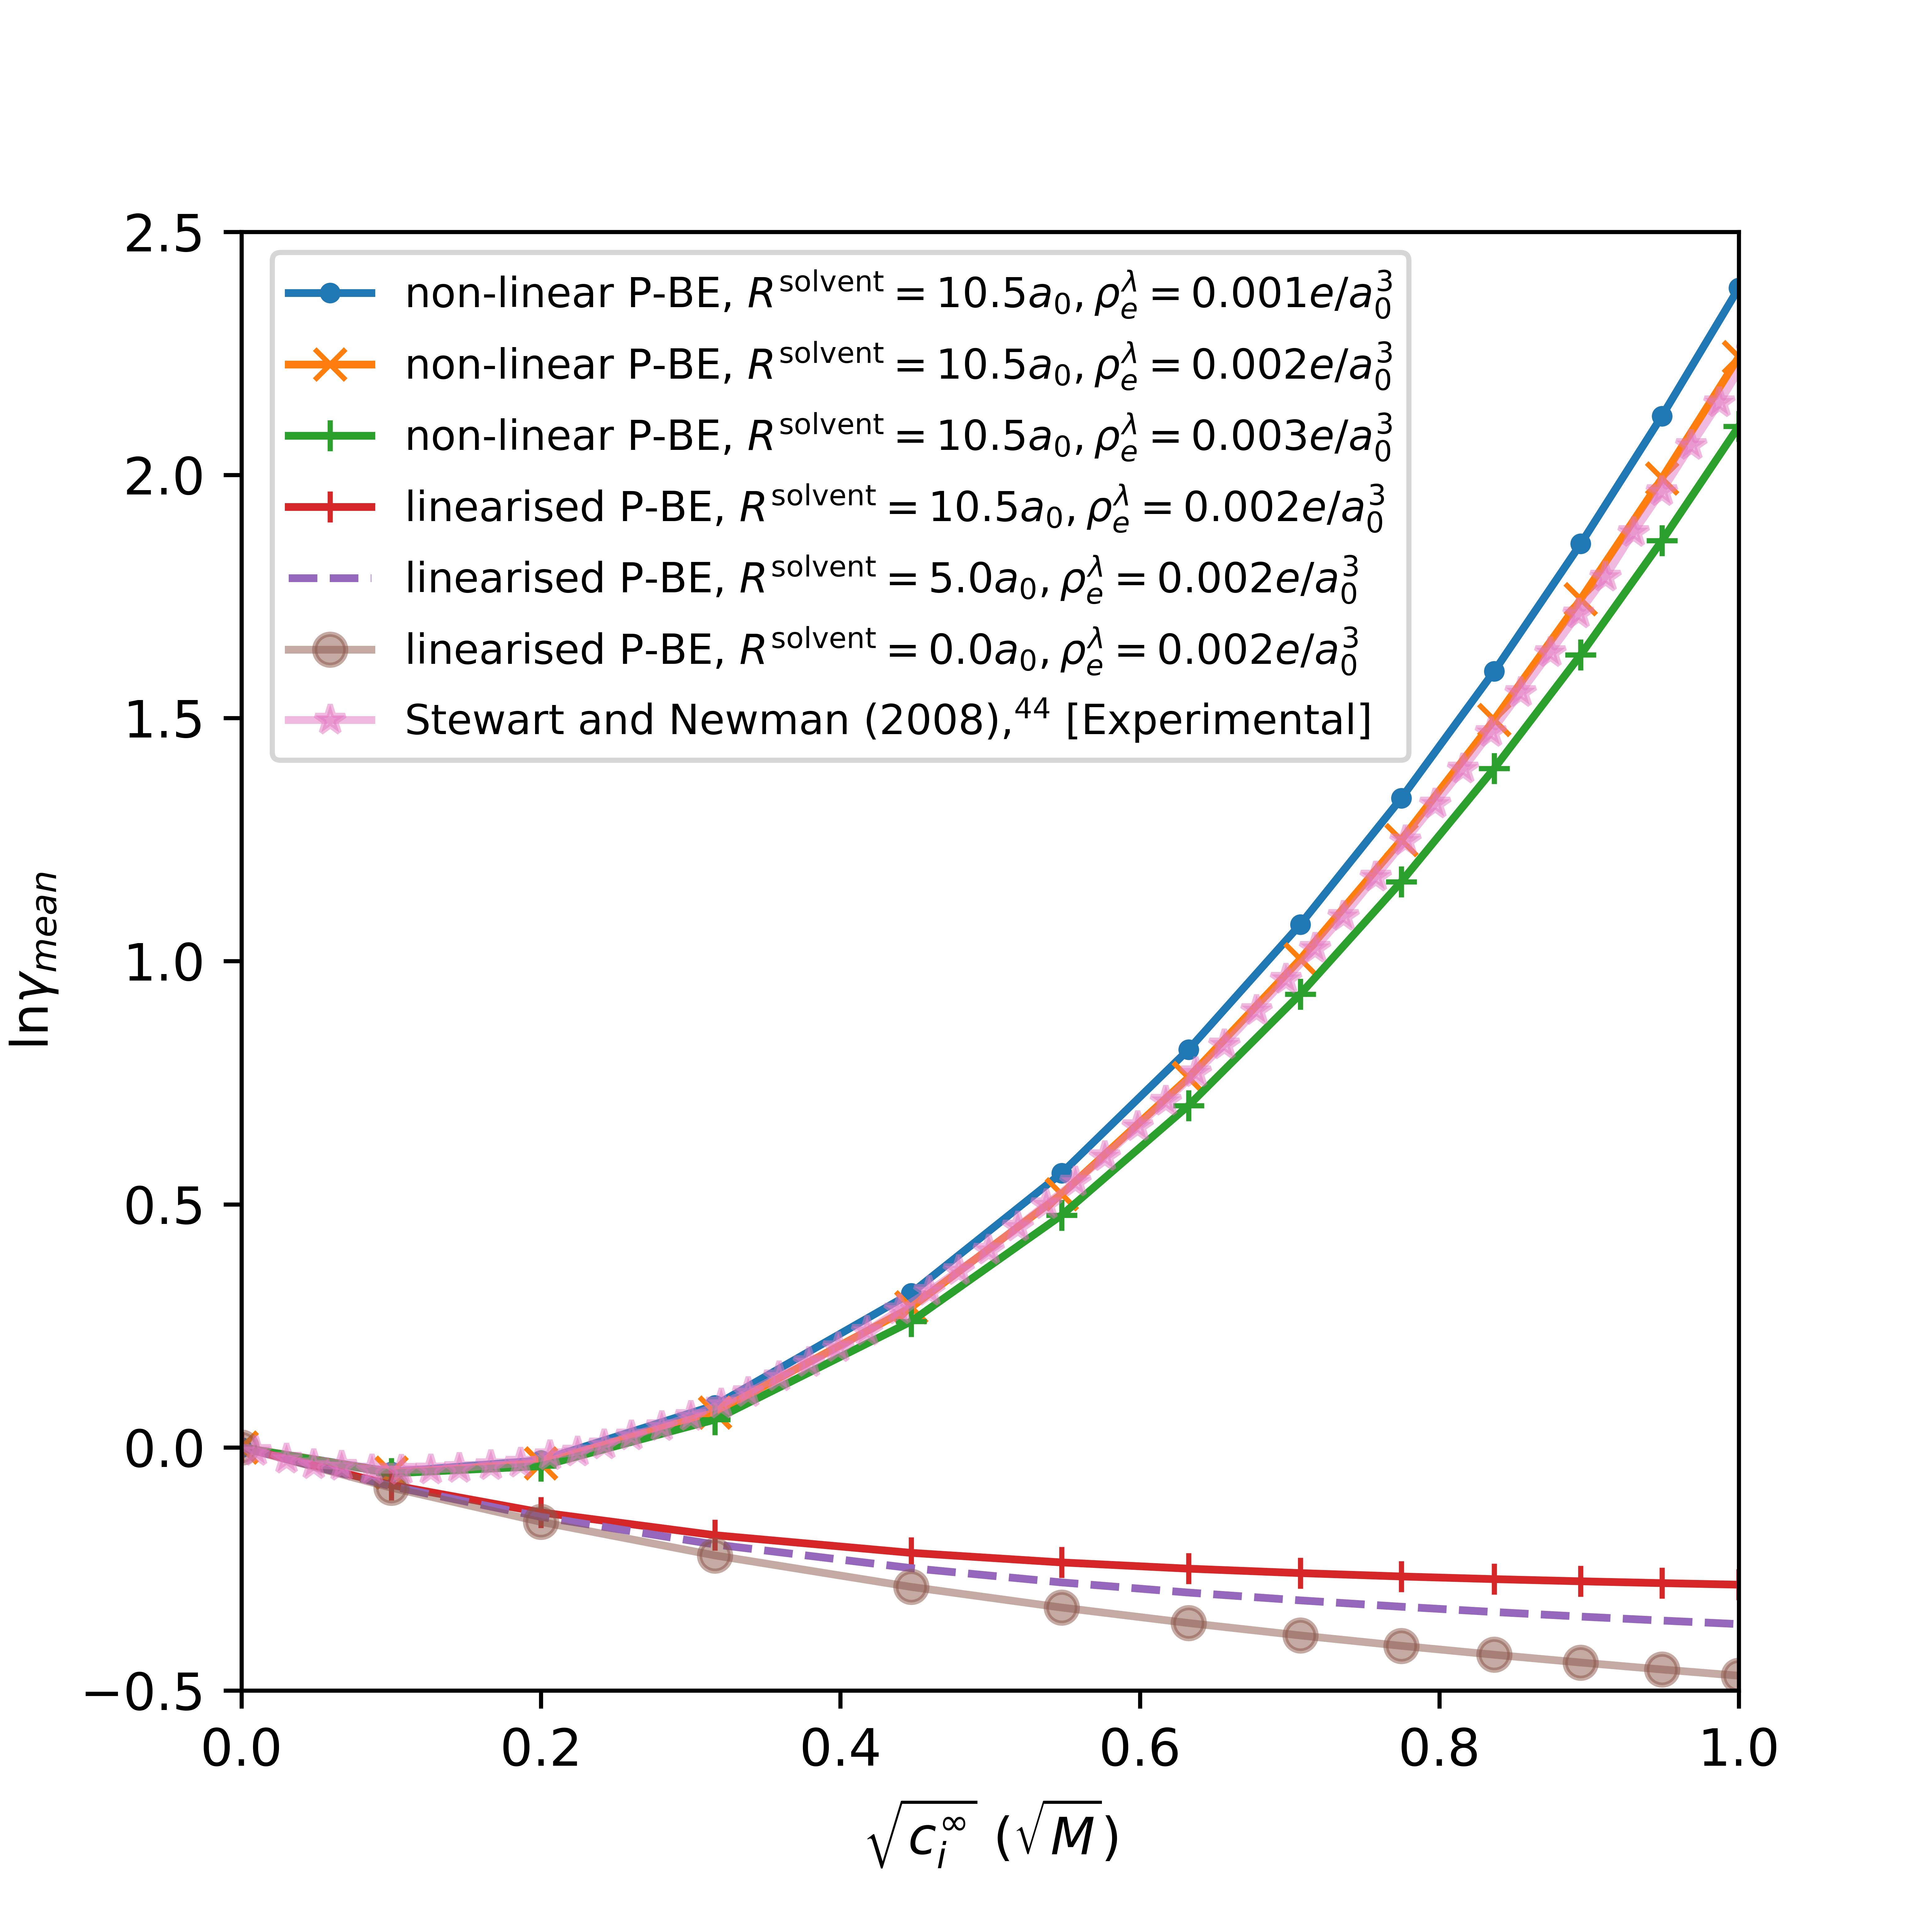
\includegraphics[scale=1]{figures/lipf6.png}
    \caption{Mean activity coefficients for LiPF$_6$ in ethylene carbonate at $T=308$~K as a function of concentration and for different values of the atomic electronic density isovalue parameter which determines the extent of the accessibility function. Calculations with the linearised approximation to P-BE are also shown. Reproduced from Ref. \citenum{Dziedzic2020}}
    \label{fig:ac}
\end{figure}
    
\subsubsection{Outlook and challenges (Arihant/Sam)}
% \begin{itemize}
%     \item challenges - interatomic potentials for classical MD
%     \item discrepancy between atomistic/continuum definition of "diffusion coefficient" in terms of parameterising for continuum modelling.
%     \item limitation of liquid electrolytes
% \end{itemize}
%end: unchanged in 30 January 2021 update

\subsection{Solid Electrolytes (Lucy/Julian/Arihant/Rana)}
\label{sec:solid_electrolytes}

\subsubsection{Introduction (Rana/Lucy/Arihant)}
%Brief History of solid electrolytes, types of solid electrolytes, types of properties which are important for batteries. Then which we will focus on in this section sulfides (using LGPS and argyrodites), oxides (Examples), composites (example).
% Possibly we can select some of the below to mention. I think the Van de Ven review covers them all, but we can focus on a few.
% Oxides - NASICONs, LISICONS, perovskites (LLTO), Li garnets, nanocomposites (ranas)
% sulfides - glass ceramics, thio-LISICON (LGPS), argyrodites.
% Others - nitrides, oxynitrides (LiPON), antiperovskites

Solid electrolytes (SE) have attracted considerable attention as an alternative to liquid electrolytes, significantly increasing the energy and power densities, improving device safety, and reducing the cost of synthesis of the battery materials. \cite{janek_solid_2016, culver_designing_2018, famprikis_fundamentals_2019, goodenough_li-ion_2013, DIRICAN201927} 
An ideal solid electrolyte material should possess  high electronic resistance, high ionic conductivity, outstanding thermal stability, strong electrochemical stability, excellent mechanical strength, and reduced interfacial resistance. \cite{han2020recent, manthiram2017} There are three different categories of solid electrolytes which are used in rechargeable batteries \cite{DIRICAN201927}: (1) Inorganic solid ceramic electrolytes, (2) Organic solid polymer electrolytes, and (3) Solid composite electrolytes. 

Solid electrolytes were discovered by Michael Faraday in the early 1830s through research on the conduction properties of heated solid sliver sulfide (Ag$_{2}$S) and lead fluoride (PbF$_{2}$) \cite{Faraday1833}. 
The use of a ceramic-based $\beta$-alumina (Na$_{2}$O$\cdot$11Al$_{2}$O$_{3}$) in high-temperature sodium-sulfur batteries in 1960s, however, was considered as a milestone in the development of batteries enabled by solid electrolytes \cite{armand2008building}. In the 1980s the Zeolite Battery Research Africa (ZEBRA) group developed the ``ZEBRA'' batteries using Na$_{2}$O$\cdot$11Al$_{2}$O$_{3}$ as the solid electrolyte. \cite{ZEBRA}
So far, the high-temperature sodium–sulfur battery has been commercialised in Japan \cite{oshima2004}, whereas the ZEBRA battery is currently being developed by the General Electric Corporation in the United States. \cite{capasso2014} 

In 1990, the Oak Ridge National Laboratory synthesised a lithium phosphorus oxynitride (LiPON) material \cite{dudney1992,bates1992}, which opened up the use of inorganic solid-state electrolytes in lithium-ion battery research. Since then, a huge number of inorganic lithium-ion conductive ceramic materials have been developed, including perovskite-type \cite{inaguma1993}, garnet-type oxides \cite{kasper1969,mazza1988}, garnet-type sulfides \cite{kennedy1986}, lithium super ionic conductor (LISICON) \cite{ivanov1988}, sodium super ionic conductor (NASICON)-like materials \cite{lang2015} and lithium-argyrodite materials. \cite{deklerk2016}

Despite recent advancement in research activities on crystalline inorganic electrolytes, they are still brittle and therefore difficult to fit into different battery shapes. Solid-state polymer electrolytes (SPEs), due to their high flexibility, can fit in any battery shape and present improved safety and stability features compared to crystalline inorganic electrolytes. \cite{DIRICAN201927} Since 1980, various high-molecular weight dielectric polymer hosts were investigated as polymer electrolytes with high conductivities for lithium batteries, such as poly(ethylene oxide) (PEO) \cite{fenton1973}, polyacrylonitrile (PAN) \cite{abraham1990,dautzenberg1994}, poly(vinylidene fluoride) (PVDF) \cite{arcella1999,kataoka2000,li2016}, poly(methyl methacrylate) (PMMA) \cite{appetecchi1995,bohnke1993} and poly(vinylidene fluoride-hexa-fluoropropylene) (PVDF-HFP) \cite{abbrent2001,park2008,yang2014}.

The ionic conductivities of most polymer electrolytes are significantly lower than those of both oxide solid electrolytes and liquid electrolytes. \cite{zhou2016} A possible solution to this limitation is to create composites by integrating nanoscale highly-conductive inorganic particulate fillers into the polymer electrolyte material. \cite{DIRICAN201927} This enhances the ionic conductivity and also improves the mechanical strength and stability of the solid-state polymer electrolytes, including the interfacial stability. \cite{D0SC03121F} Here, heterogeneous doping increases the ionic conductivity as a result of increasing interfacial regions between an inert solid phase, such as silica or alumina or boron oxide particles and an electrolyte. \cite{uvarov2011} A wide range of inorganic solid composite electrolytes have previously been studied, based on oxides (Li$_{2}$O:Al$_{2}$O$_{3}$ \cite{B300908D}, Li$_{2}$O:B$_{2}$O$_{3}$ \cite{Heitjans_2003,Indris2000,Indris2002}), hydrides (LiBH$_{4}$:SiO$_{2}$ \cite{blanchard2015}), halides (LiI:Al$_{2}$O$_{3}$ \cite{liang1973}, LiI:SiO$_{2}$ \cite{phipps1983}, LiF:Al$_{2}$O$_{3}$ \cite{uvarov1992}), and sulfides (Li$_{2}$S:SiS$_{2}$ \cite{pradel1986}). 

The high ion conductivities of liquid electrolytes have, thus far, been unreachable for solid electrolytes, however, research efforts over the last decade have presented a limited number of promising candidates with high ionic conductivities ($>$1 mS cm$^{-1}$) as a potential competitive to liquid electrolytes.\cite{kanno_synthesis_2000,murayama_synthesis_2002,murayama_material_2004,minafra_influence_2019,bron_li_2013,whiteley_empowering_2014,huang_superionic_2019,yamane_crystal_2007,homma_crystal_2011} Figure \ref{fig:conductivity} presents a plot by \citeauthor{Kamaya2011} with the ionic conductivities of most currently known solid electrolytes.

In this section, we review atomistic modelling investigations into the structure-property relationships in selected solid-state electrolytes; Li$_{10}$GeP$_2$S$_{12}$ (LGPS), lithium argyrodites, and Li$_7$La$_3$Zr$_2$O$_{12}$ (LLZO) which belong to the inorganic solid ceramic electrolyte type and Li$_{2}$O:B$_{2}$O$_{3}$ materials which belong to the oxide based solid composite type. A particular focus is given on the ion transport mechanism in those materials which is important for reaching high conductivities, a key property of battery materials. Finally, we take a more detailed look at the interface of solid electrolytes with the electrodes, and discuss the challenges and outlook for future atomistic modelling investigations.

\subsubsection{Sulfides (Arihant/Lucy)}
There are a larger number of computational studies of sulfides which partly related to a recent increase in newly discovered crystalline sulfide superionic conductors. Sulfides also tend to have comparatively lower intrinsic electrochemical and chemical stability, which has stimulated interest for understanding the interfacial interactions within batteries. \cite{Xiao2020interfacerev} The sulfide group encompasses a range of sulfide based solid electrolytes, including, glass ceramics \cite{minami2006recent}, argyrodites \cite{bai2020research}, and thio-LISICONs \cite{minafra2020two}. Some of the most promising SEs to emerge in recent years include the Li$_{10}$GeP$_2$S$_{12}$ (LGPS) \cite{Bhandari2016,Kamaya2011,Mo2012} and the Li-argyrodite (Li$_6$PS$_{5}X$, $X$=Cl,Br,I) \cite{kraft2018,deiseroth_li6ps5x_2008,deklerk2016,kraft2017,minafra2018,adeli2019} families of superionic conductors.

\textbf{LGPS}
The crystal structure and the phenomenal ionic conductivity (12 mS/cm at room temperature) of Li$_{10}$GeP$_2$S$_{12}$ was reported by \citeauthor{Kamaya2011}, see Fig.~\ref{fig:conductivity}. \cite{Kamaya2011} \citeauthor{Kamaya2011} determined that diffusion in LGPS is anisotropic where the $c$ directional motion is predominant over that in the $ab$ plane, with an overall energy barrier for Li diffusion being 0.24 eV. The discovery was followed by an ab-initio MD study by \citeauthor{Mo2012}, who determined an average energy barrier of 0.17 eV along the $c$ channel and 0.28 eV in cross channel direction, i.e. along the $ab$ plane.\cite{Mo2012} A Further computational study by \citeauthor{Xu2012one} revealed that the Li atoms move along the $c$ channels in a cooperative way, instead of through the nearest neighbor hops, due to the large coulombic repulsion between them.\cite{Xu2012one} \citeauthor{Adams2012} performed a molecular dynamics study and predicted the presence of additional Li sites which would provide diffusion along the $ab$ plane.\cite{Adams2012} The additional sites could change the diffusion scenario altogether, by not only changing the occupancies of Li in the $c$ channel, but also by providing a diffusion mechanism involving $ab$ plane. Later, \citeauthor{Kuhn2013a} confirmed the presence of these additional sites experimentally by performing single crystal XRD.\cite{Kuhn2013a} The interesting discovery of additional sites has opened up the possibility of cross-channel mechanisms of ion movement. \citeauthor{Kuhn2013b}, in a further study, reported that the diffusion in LGPS is more or less isotropic with an overall activation energy barrier of 0.22 eV.\cite{Kuhn2013b}

\citeauthor{Bhandari2016} performed a first-principles DFT study of Li diffusion energy barrier in LGPS via the nudged elastic band (NEB) method, taking into account the fractional occupancies leading to variable $c$ channel Li populations, variable chemical environments surrounding Li, and all possible migration mechanisms.\cite{Bhandari2016}  They found that the Li diffusion is neither purely $c$ directional nor purely along the $ab$ plane, but there exists a correlated mechanism of motion along $c-ab$ which critically controls the degree of anisotropy of Li diffusion in LGPS. The energy barriers for different mechanisms of Li-diffusion are shown in Fig. \ref{fig:lgps}, which suggests that the correlated hop has the lowest energy barrier. %This correlated mechanism of Li-diffusion could not be deciphered from the experimental data or MD data alone, as these methods can only isolate diffusivities along particular directions. 
\citeauthor{Bhandari2016} further performed a statistical average of all diffusion energy barriers, taking into account the formation energy of various Li configurations and predicted an overall energy barrier of 239 meV, which is in close agreement with experiments.\cite{Kamaya2011} Thus, the first-principles approach not only explained the overall diffusivities and energy barriers, but also gave insight into the underlying mechanism behind the fast Li diffusion in LGPS and resolved the discrepancy about the anisotropy of Li diffusion in this compound.

\begin{figure}
    \centering
    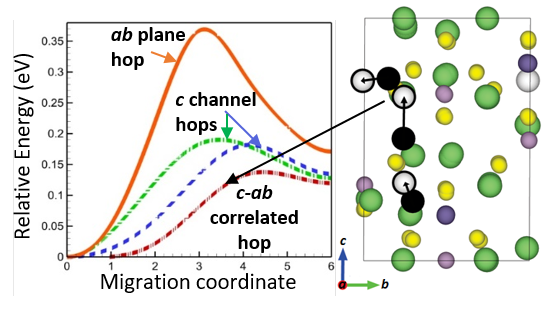
\includegraphics[scale=1.2]{figures/lgps.png}
    \caption{Energy barrier for Li-ion diffusion in LGPS solid electrolyte calculated using NEB method. Reproduced from Ref. \citenum{Bhandari2016}}
    \label{fig:lgps}
\end{figure}

\textbf{Lithium argyodites}, Li$_6$PS$_{5}X$ ($X$= Cl,Br,I) can reportedly reach ionic conductivities of up to $10^{-2}$ Scm$^{-1}$. \cite{deiseroth_li6ps5x_2008} While Li$_6$PS$_{5}$Cl and Li$_6$PS$_{5}$Br exhibit high ionic conductivities of $10^{-3}$ Scm$^{-1}$ at room temperature, Li$_6$PS$_{5}$I has considerably lower conductivitives of $10^{-6}$ Scm$^{-1}$.The three orders of magnitude difference is surprising as the identical crystal structures suggest the same Li diffusion pathways exist in all systems. Another intriguing aspect is that the conductivity trend runs counter to other families of SEs, such as LGPS, where larger, more polarisable and less electronegative anions are linked with increased ionic conductivites. \cite{bachman2016inorganic}

Understanding which properties and mechanisms influence the conductivity is essential to obtaining higher ionic conductivities and improving battery performance. Material stoichiometry, anion/cation disorder, and doping, have all been shown to influence conductivities. The effect of these can be difficult to deconvolve in many materials as they are intrinsically coupled in experimental systems. This is where computational analysis can provide vital insight, allowing deconvolution of coupled properties and the roles they play in the diffusion process.

A particularly interesting aspect of the Li-argyrodites is the diffusion topology, which comprises of interconnected Li$_6$S cages, with anions arranged at 4a, 4c, and 16e Wyckoff positions and Li arranged over type 1, 2, 4, and 5 tetrahedra.\cite{kuhs1979} Lithium mainly occupies type 5 tetrahedral sites in $x$(Li)=6 argyrodites, with occupation of non-type 5 sites only recently observed experimentally. \cite{ohno2019further,gautamengineering} Computational studies however have previously predicted occupation of non-type 5 sites, showing lithium distributed over tetrahedral types 5, 2, and 4. \cite{deiseroth_li6ps5x_2008, Minafra2020, morgan2020mechanistic}

Li hopping within these cages, while effectively barrier-less, does not contribute to long-range diffusion. In fact, a combination of inter-cage and intra-cage hopping is needed, with occupation of non-type 5 sites and transitions between all adjacent site types to achieve long-range diffusion. This is shown schematically in Figure~\ref{fig:diffusion_pathways} showing the connectivity between the Li tetrahedral sites. AIMD simulations have shown that cation and anion substitution \cite{ohno2019further,deklerk2016}, anion site disorder \cite{gautamengineering,morgan2020mechanistic}, and lithium concentration \cite{Deng2017, yu_superionic_2020, Feng_2020}, all influence the ionic conductivity.

\begin{figure}
    \centering
    
\includegraphics[scale=0.65]{figures/diffusion_pathways.pdf}
    \caption{(a) Possible Li diffusion pathways in Li-argyrodites involving types 2, 4, and 5 tetrahedra for long range diffusion. Ref. \citenum{morgan2020mechanistic}}
    \label{fig:diffusion_pathways}
\end{figure}

The influence of anion substituent concentration on conductivity is currently uncertain, with research by \citeauthor{deklerk2016} determining excess Cl in Li$_5$PS$_4$Cl$_2$ resulting in similar conductivities to Li$_6$PS$_5$Cl \cite{deklerk2016}, in contrast to research by \citeauthor{yu2019tailoring} and \citeauthor{Feng_2020} concluding excess Cl improved Li conductivity. \citeauthor{yu2019tailoring} determined the highest conductivity was produced by Li$_{5.7}$PS$_{4.7}$Cl$_{1.3}$ (6.4 mS cm$^{-1}$), \cite{yu2019tailoring,yu_superionic_2020} while \citeauthor{Feng_2020} determined this to be Li$_{5.3}$PS$_{4.3}$Cl$_{1.7}$ (17 mS cm$^{-1}$). \cite{Feng_2020} \citeauthor{Feng_2020}, however, presented alternative, or coupled, reasoning for this increased conductivity. Drawing from previous studies \cite{adeli2019,zhou_solvent-engineered_2019} they propose the increased Cl content amplified the anion disorder in the system, which is the underpinning cause of the higher conductivities.

\subsubsection{Oxides (Julian/Rana)}
\label{sec:se_oxides}

% \begin{itemize}
%     \item Intro
%     \item LLZO (Julian)
%     \item Nanocomposites (Rana)
% \end{itemize}

\textbf{LLZO} Cubic Li$_7$La$_3$Zr$_2$O$_{12}$ (c-LLZO) shows its promise as a solid electrolyte by fulfilling a number of criteria essential for this role. It has a high Li-ion conductivity (\(3\times 10^{-4}\,\mathrm{Scm}^{-1}\))\cite{Murugan2007}, a high shear modulus (59\,GPa)\cite{Ni2012}, and the largest thermodynamic stability window against lithium metal\cite{Zhu2016, Binninger2020} of current solid electrolyte materials. However, c-LLZO is not a stable phase at room temperature.\cite{Geiger2011} At lower temperatures (\(<150 ^\circ C\)) a phase transition occurs forming the much less ionically conductive tetragonal LLZO (t-LLZO) phase.\cite{Geiger2011} c-LLZO can be retained by Al doping on lithium sites.\cite{Geiger2011, Rangasamy2012}

However, lithium dendrite growth has proven to be a problem. It has caused short circuits in LLZO cells after relatively short periods of use \cite{Ren2015,Sudo2014}. This growth has been observed directly by \citeauthor{Cheng2017}, who found that this process occurs mostly through grain boundaries.\cite{Cheng2017} \citeauthor{Kim2020} corroborated this observation and investigated the use of an interlayer buffer as a means to restrict Li propagation through grain boundaries.\cite{Kim2020}

\citeauthor{Monroe2004} predicted, through the classical kinetic modelling of an electrode-solid electrolyte interface, increasing surface stability with increasing shear modulus for solid electrolytes.\cite{Monroe2004, Monroe2005} It is therefore surprising that dendrite growth occurs in LLZO which has respectively large shear modulus compared to other solid electrolytes. However, the authors do note that their models do not account for fracturing of a brittle material.

The potential of this material coupled with its dendrite issue has led to a number of attempts to model this formation\cite{Canepa2018, Tian2018, Gao2020}. \citeauthor{Tian2018} used DFT (cf. section \ref{sec:dft}) to investigate dendrite growth. \cite{Tian2018} The total density of states (TDOS) of the lowest energy surface slab and bulk structures were compared for c-LLZO and t-LLZO. t-LLZO forms at the surface of bulk c-LLZO even with Al-doping\cite{Ma2016, Rettenwander2018}. Comparison of the TDOS revealed there were extra states in the band gap for the slab structures. This may allow electrons to be trapped on the surface of LLZO. The electrons localisation on the surface was found by adding electrons to the structures and comparing the charge density change. Localisation occurred primarily around Li$^+$ and La$^{3+}$ ions on the surface. The lithium reduction product was found to be more favourable. \citeauthor{Tian2018} concluded that the trapping of electrons on the surface led to the nucleation of lithium metal. This could lead to growth through grain boundaries and pores in the LLZO eventually forming dendrites\cite{Ren2015}, Fig. \ref{fig:tian2020}. The same tests were performed Li$_2$PO$_2$N (LiPON) no electron trapping was found to occur indicating it may make a suitable coating to prevent dendrite and t-LLZO formation (cf. section \ref{sec:interface_stability}).

\begin{figure}[H]
    \centering
    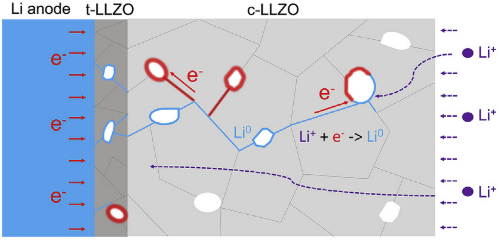
\includegraphics{figures/tian_grain_growth.png}
    \caption{Schematic showing Li metal formation (blue) along grain boundaries and pores due to electron accumulation (red) combining with Li$^+$ as they move through the electrolyte. From Ref. \citenum{Tian2018}}
    \label{fig:tian2020}
\end{figure}

This theory for the dendrite growth mechanism is contradicted by \citeauthor{Gao2020} who attributed it to the under-coordination of Zr present on some of the stable surfaces of LLZO .\cite{Gao2020} This under-coordination can lead to inhomogenous Li depletion which has been linked to Li metal depostion and dendrite formation.\cite{Tsai2016} The apparent rift between these two papers stems from the choice of surface. \citeauthor{Tian2018} argue that lithium and lanthanum rich surfaces are more stable based upon the the research conducted by \citeauthor{Thompson2017}, where DFT calculations on 6 different LLZO slabs for the 100 and 110 planes, was performed.\cite{Thompson2017} In contrast, \citeauthor{Gao2020} drew upon results presented in several methods\cite{Thompson2017, Canepa2018, Yu2016a} and performed DFT calculations on a wider range of surfaces, finding 100 and 001 surfaces the most stable. They agreed with the findings of \citeauthor{Tian2018} with respect to Li and La rich surfaces being the most stable. However, \citeauthor{Gao2020} analysed the Li-LLZO interface using the CALYPSO interface structure prediction method\cite{Wang2012, Gao2019}, which calculated the interface formation energies. They found the Zr-rich surfaces tended to form the most stable interfaces with the Li anode. Zr-caused interfacial degradation has been observed experimentally by \citeauthor{Zhu2019} \cite{Zhu2019}.

Some experiments have suggested a primary cause of dendrite growth is a non-uniform distribution of current on the surface causing Li reduction.\cite{Han2019_dendrite, Aguesse2017} A pre-print by \citeauthor{squires_2020} models electronic conductivity in LLZO to probe how important surface current is to dendrite formation.\cite{squires_2020} DFT calculations were performed and the results fed into a novel workflow to find the electronic conductivity. At room temperature, bulk c-LLZO was found to have negligible electron/electron-hole concentrations indicating that bulk defects are not a significant factor in dendrite growth. However, their model has not been applied to other forms of defects such as grain boundary and surface effects. 

\citeauthor{Xu2012} analysed the Li-ion migration path through LLZO using DFT with the nudged elastic band (NEB) method (cf. section \ref{sec:methods_neb}). Two migration paths were observed, depending on Li concentration.\cite{Xu2012} Low Li concentration (around Li$_5$La$_3$Zr$_2$O$_{12}$) led to a higher energy, single hop, migration path. At higher Li concentrations (around Li$_7$La$_3$Zr$_2$O$_{12}$), led to a lower energy, two hop, migration path.

\citeauthor{Burbano2016} used classical molecular dynamics (cf. section \ref{sec:molecular_dynamics}) to find a more robust description of the ion transport mechanism.\cite{Burbano2016} Interatomic potentials were found using a hybrid DFT functional. The difference in ionic conductivity between t-LLZO and c-LLZO were compared. They found the longer time scale of classical MD allowed the observation of a large sample of diffusion events in both LLZO structural forms. Diffusion events in t-LLZO were less common and mostly involved exactly 8 Li ions. The significance of this is 8 Li events correspond to the cyclic movement of Li ions about a ring of 12 octahedral an tetrahedral sites in t-LLZO. This cyclic mechanism results in no net diffusion of Li and hampers the ability of t-LLZO to conduct ions.

Previous AIMD (cf. section \ref{sec:molecular_dynamics}) investigations of the transport mechanism in LLZO have been conducted. The smaller time scale led to some key disagreements about the transport mechanism in c-LLZO.\cite{Meier2014, Jalem2013, Burbano2016}

More recently \citeauthor{Bonilla2019} applied classical MD to investigate the ionic conductivity in Al-doped LLZO.\cite{Bonilla2019} DFT calculations had revealed Al doping reduces the energy barrier for Li-ions to move between octahedral and tetrahedral sites.\cite{Rettenwander2014, Rettenwander2016} \citeauthor{Bonilla2019} supported this by finding that an increase in conductivity in t-LLZO was due to the Al forcing Li ions into previously inaccessible tetrahedral sites. It was also found Al doping in c-LLZO led to a slight decrease in conductivity. They attributed this to the tendency for Al to "trap" Li ions close to the dopant.

A recent review of experimental and computational techniques used to probe ion transport mechanisms can be found in ref. \citenum{Gao2020_ion_transport}.

\citeauthor{Sharafi2017} investigated the low wettability of Li on LLZO using DFT.\cite{Sharafi2017} They found the calculations to be in good agreement with the experiments conducted within the paper.

Atomistic modelling has proven useful in probing the properties of LLZO. It has revealed insights in dendrite growth, ion transport, thermodynamic stability, electronic conductivity and wettability. Atomistic modelling has moved away from the bulk material and is looking at the interfaces formed with LLZO and other solid electrolytes (see sec. \ref{sec:interface_stability}) as well as investigating the effectiveness of various coatings in mitigating some of the unfavourable properties outlined in this section. 

\textbf{Oxide Nanocomposites} Due to attractive mechanical, electrical, optical, and magnetic properties nanocomposite oxide materials represent a new generation of advanced materials. \cite{uvarov2011,Heitjans_2003} They often show enhanced conductivity compared to the single-phase ceramic oxides which makes them suitable candidates as electrolytes for future solid state batteries. For example, Li$_2$O:B$_2$O$_3$ \cite{Heitjans_2003,Indris2000,Indris2002} and Li$_2$O:Al$_2$O$_3$ nanocomposites \cite{B300908D} have higher ionic conductivities than nanocrystalline Li$_2$O, although B$_2$O$_3$ and Al$_2$O$_3$ are insulators. The ionic conductivity shows a maximum at about 50 \% of B$_2$O$_3$/Al$_2$O$_3$ content. This surprising behaviour was attributed to the increased fraction of structurally disordered interfacial regions and the enhanced surface area of the nanosized particles \cite{Heitjans_2003}. The oxide nanocomposites contain three types of interfaces, as presented in Fig.~\ref{fig:LBO} (a): interfaces between the ionic conductor grains (green lines), between the insulator grains (black lines), and between the ionic conductor and the insulator grains (red lines). The latter can lead to surprising effects in the conductivity of composite materials. In this case, the highly conducting interface region can act as a bridge between two Li$_2$O grains not in direct contact with each other, opening up additional paths for Li ions. The conductivity enhancement in the interfacial regions may have different origins, e.g. the formation of space charge layers, an enhanced concentration of dislocations, or defects or the formation of new phases.

\begin{figure}
    \centering
    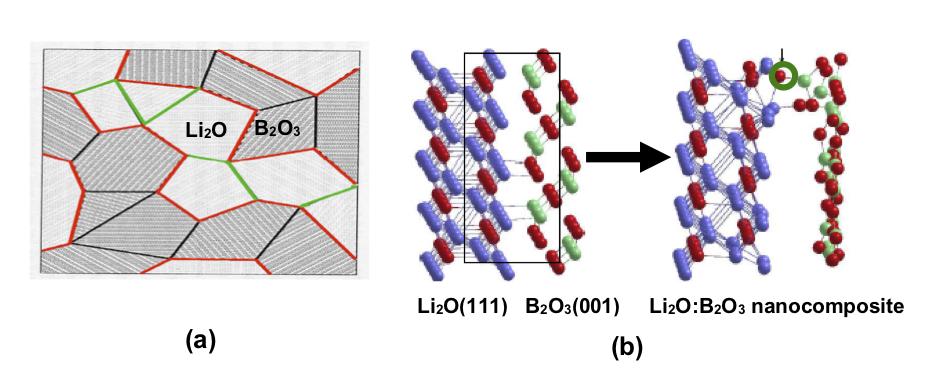
\includegraphics[scale=1]{figures/Islam-Fig-Li2O-B2O3.png}
    \caption{(a) Schematic diagram of Li$_2$O and B$_2$O$_3$ interface (Reproduced from ref. \citenum{Heitjans_2003}). (b) Atomistic model of Li$_2$O:B$_2$O$_3$ nanocomposite ref. \citenum{Rana-JPCM-2012}.}
    \label{fig:LBO}
\end{figure}

\citeauthor{Rana-PRL-2007} studied the interface of Li$_2$O:B$_2$O$_3$ nanocomposite by modelling a combination of two favorable surfaces of Li$_2$O and B$_2$O$_3$ using HF/DFT Hybrid approach. \cite{Rana-PRL-2007,Rana-JPCM-2012} After full structural optimisation, it was observed that Li--O bonds are weakened and simultaneously B--O bonds are formed at the boundary between the two surfaces, Fig. \ref{fig:LBO} (b). An oxygen atom from the Li$_2$O surface (marked by a green circle) is pulled from the surface layer towards a neighboring boron atom of the B$_2$O$_3$ surface. This preference of oxygen bonding with B (or Al in Li$_2$O:Al$_2$O$_3$) plays a key role in generating low-coordinated Li. As a consequence of this dislocation, the coordination of a Li atom in the second layer is reduced from four to three. 

The defect properties were investigated in the interface region. It was observed that the removal of surface oxygen from Li$_2$O is responsible for the increased vacancy defect concentration in Li$_2$O:B$_2$O$_3$ (or Li$_2$O:Al$_2$O$_3$) nanocomposite materials. Therefore the nanocomposites of ionic compounds (containing weakly bound and therefore mobile cations) with highly covalent compounds (with strong metal- or nonmetal-oxygen bonds) are in general promising candidates for high ionic conductivity. The model calculations showed that the most likely mechanism for Li$^+$ migration was in a zigzag pathway rather than in a straight line along a direction parallel to the interface plane. 

The average calculated activation energy for Li$^+$ migration in the Li$_2$O:B$_2$O$_3$ interface (0.28 eV) \cite{Rana-PRL-2007,Rana-JPCM-2012} is similar to the experimental values of bulk Li$_2$O (0.31 eV) \cite{Heitjans_2003}, Li$_2$O:B$_2$O$_3$ ($0.34 \pm 0.04$ eV) \cite {Indris2002} and Li$_2$O:Al$_2$O$_3$ ($0.30 \pm 0.02$ eV) \cite{B300908D} nanocomposites. According to the defect formation energies, the interface region of Li$_2$O:B$_2$O$_3$ nanocomposites contains higher concentrations of both Li vacancies and Frenkel defects than bulk Li$_2$O and the Li$_2$O surfaces. \cite{Rana-PRL-2007,Rana-JPCM-2012} Therefore the experimentally observed enhanced Li mobility in the Li$_2$O:B$_2$O$_3$ interface region is thermodynamically and not kinetically controlled. Models as proposed in that study allowed a direct simulation of the defect formation and ion mobility at atomic scale without any experimental input. They provided a deep insight into the local bonding situation at the interface of oxide nanocomposites which was difficult to obtain from experiments.


\subsubsection{Interface stability (Julian)}
\label{sec:interface_stability}

Atomistic modelling has proven to be a useful asset when examining solid electrolyte interfaces as probing the interfaces experimentally is often difficult\cite{Xu2018exp}.An in-depth experimental and computations review on solid electrolyte interfaces is given by \citeauthor{Xiao2020interfacerev} \cite{Xiao2020interfacerev} Here, we focus on an overview of the atomistic modelling contributions to the investigation of these interfaces. 

It was widely reported in both experiment\cite{Liu2013, Han2015} and theory\cite{Mo2012} that certain solid electrolytes have an electrochemical stability window against a Li anode between 0--5 V.\cite{Kamaya2011, Thangadurai2005, Liu2013} \citeauthor{Mo2012} reported a 3.6 eV band gap from a DFT calculation (cf. section~\ref{sec:dft}) for LGPS.\cite{Mo2012} They attributed this to the extra stability observed in experiment to the passivisation phenomenon forming a SEI at the interface of the anode-electrolyte.\cite{Kobayashi2008}
More recent work has questioned this high stability window. \citeauthor{Zhu2015} demonstrated using DFT, that the stability windows, particularly of sulfides, are far smaller than originally thought (fig.~\ref{fig:se_stab}).\cite{Zhu2015} 

\begin{figure}[H]
    \centering
    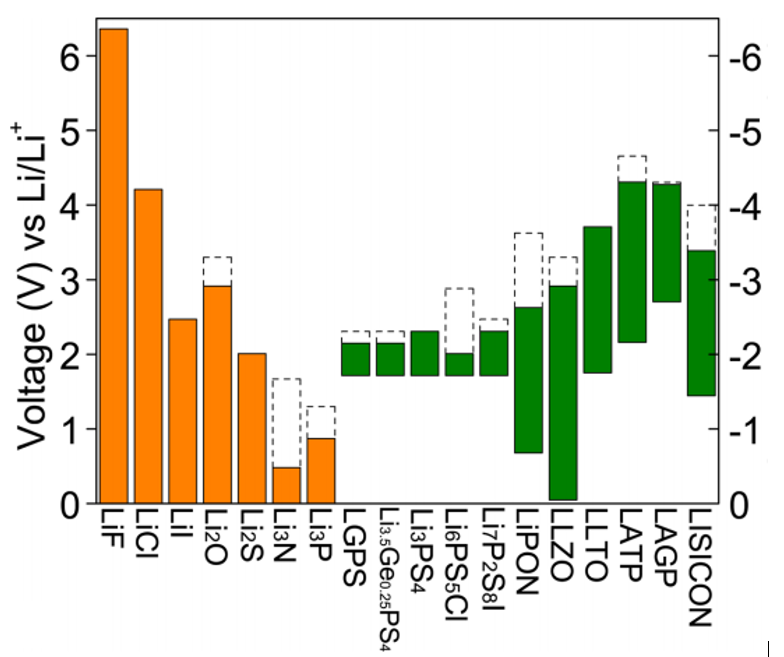
\includegraphics[scale=0.5]{figures/SE_voltage_stability.png}
    \caption{A comparison of the voltage stability windows for a selection of solid electrolytes (green) and the binary compounds that often form upon decomposition of the solid electrolyte (orange). The dashed line represents the oxidation potential to fully delithiate the material. From Ref. \citenum{Zhu2015}}
    \label{fig:se_stab}
\end{figure}

The significance of the reduced thermodynamic window is that it places a higher importance on the interphase layer formation. In general \citeauthor{Zhu2015} found these solid electrolytes to be unstable with respect to Li metal at low and high voltages with the exception of LLZO that appears to be kinetically stabilised at low voltage as it has an unfavourable reduction energy of only -0.02 eV per atom. Any potential outside of the solid electrolyte's thermodynamic stability window (fig. \ref{fig:se_stab}) results in decomposition into lithium binary compounds. This is problematic for germanium and titanium containing compounds as they form electronically conductive alloys.\cite{Zhu2015} This renders the proposed passivation process impossible\cite{Mo2012, Zhu2015} as this degradation would be sustained throughout the bulk cycling severely limiting the efficacy of these materials as electrolytes. Other solid electrolytes face different problems. As explained in sec. \ref{sec:se_oxides}, LLZO forms the far less ionically conductive tetragonal LLZO at the surface. The Li-LiPON and Li-argyordites interfaces were reported to degrade favourably, forming an ionically conductive and electronically insulative interphase consisting of Li2O, Li2S, Li3P, Li3N, and LiI.\cite{Zhu2015} 

Further study by \citeauthor{Zhu2016} sought to investigate the mechanism behind the degradation/instability at the surface.\cite{Zhu2016} In order to probe this they looked at several solid electrolytes (LGPS, LLZO, LiPON, NAISICON-type, LLTO) and calculated the chemical stability, electrochemical stability and the equilibrium conditions at the interfaces. Examining the cathode-electrolyte interface, using lithium cobalt oxide (LCO), a similar pattern emerged. Oxides were far more stable than their sulfide counterparts. However, LLTO and LATP had the best electrochemical stability against LCO. LLZO still performed well. 

Studies looking into the interfacial resistance have been conducted. \citeauthor{Tateyama2019} attributed the main source of the resistance to the electric double layer which in liquid electrolytes consists of a capacitance and diffusion layer.\cite{Tateyama2019} They investigated this by using the CALYPSO method to find low-energy surfaces\cite{Gao2019} as they could not use typical Molecular Dynamics methods, due to computational costs, to probe the interface as done with liquid electrolytes (see sec. \ref{sec:Liquid_electrolytes}). Once stable interfaces were found, the lithium chemical potential in the Helmholtz layer could be found. This corresponds to the negative of the Li ion vacancy formation energy. These energies correspond to where the the lithium will move from the electrode to the electrolyte first. These sites depleting first upon charging can be a source of interfacial resistance. 

A study by \citeauthor{Lepley2015} used DFT to investigate the interface energies between the Li electrode and the compounds that make up the interphase layer of the electrolyte.\cite{Lepley2015} They defined the interface energy as 

\begin{gather}
    \gamma_{ab}(\Omega)=\frac{E_{ab}(\Omega,A,n_a,n_b)-n_aE_a-n_bE_b}{A}
\end{gather}

where $\Omega$ is the interface configuration of atoms, $E_{ab}$ is the energy of the complete system, $E_x$ is the bulk energy per for formula unit and $A$ is the surface energy. Because the interface energy is intensive, calculating larger systems will give a converging value for $\gamma_{ab}$.

\begin{gather}
    \lim_{\Omega_s \rightarrow \Omega} \left[\gamma_{ab}(\Omega_s)\right]=\gamma_{ab}(\Omega)
\end{gather}

$\Omega_s$ is the atomic configuration in a sample of the interface volume. Because the exact matching of lattice constants between interfaces is unlikely a semi-coherent interface is considered. This meant that lattice strain needed to be accounted for. By finding the structure with the lowest overall lattice energy and explicitly accounting for the lattice strain the most probable interfaces could be found. The Li/Li$_3$PO$_4$, Li/Li$_2$O and Li/Li$_2$S interfaces were found to be stable and Li/Li$_3$PS$_4$ interface, unstable.

In response to the apparent poor stability of most solid electrolytes many studies have attempted to simulate the effect of coating the electrolyte with an oxide layer\cite{Zhang2020directvis, Xiao2019coat, Tian2018}. \citeauthor{Tian2018}'s methods are discussed in sec. \ref{sec:se_oxides}. They identified LiPON as a suitable coating material for LLZO by comparing the bulk and surface DOS\cite{Tian2018}. They found no extra states on the surface structure, so concluded that no electron trapping would occur (the primary mechanism that they attributed to dendrite formation). In a recent paper by \citeauthor{Sang2020} they proposed a artificial SEI between the Li anode and the solid electrolyte composed of a Li$_{3a_b}$N$_a$X$_b$ compound, where X is a halide.\cite{Sang2020} 
This material was investigated computationally by screening stable and metastable structures using the USPEX structure prediction software.\cite{Glass2006, Oganov2006} The dynamic stability of the stable structures was found by analysing the phonon frequency spectrum by using the PHONOPY package.\cite{Parlinski1997, Togo2008} The temperature-dependant ionic transport properties were found using ab-inito molecular dynamics (AIMD). 
(see sec.\ref{sec:molecular_dynamics}) 
Phase diagrams for various atomic configurations were then constructed through Alloy-Theoretic Automated Toolkit (ATAT) which uses the cluster expansion method (see sec. \ref{sec:cluster_expansion}).\cite{Hart2008, VandeWalle2002} Through these various computational techniques \citeauthor{Sang2020} found that Li$_6$NCl$_3$ to have the most favourable properties for use with sulfide-based solid electrolytes such as LGPS. 

Electrolyte, cathode and anode coatings is a very active and broad area of theoretical and experimental research. To address all major publications pertaining to coatings would fall outside the scope of this review. 

Our understanding of solid electrolyte interfaces and their stability has benefited from atomistic simulation. Given the intrinsic difficulty associated with studying surfaces experimentally, a greater responsibility is placed on these simulations for battery development. However, the limited size under which high accuracy atomistic simulations can be conducted can mean certain important properties related to interface stability are missed (e.g. the electric double layer\cite{Tateyama2019}).

\subsubsection{Outlook and challenges (Julian/Lucy)}
\label{sec:outlook_electrolytes}
% \begin{itemize}
%     \item Dendrite formation
%     \item lattice mismatch between SE and electrodes
%     \item simulation too small or too high level to model the electric double layer
% \end{itemize}

The drive for the development of commercialised all-solid-state batteries has been intense, with the electric vehicle industry being at the forefront of promoting this.\cite{Woods_2021} Although solid-state batteries can offer high gravimetric energy (250 Wh kg$^{-1}$) and volumetric energy (700 Wh L$^{-1}$), the slow kinetics can impair the fast discharge and charge performance. With solid electrolytes intended to replace both the separator and liquid electrolyte in conventional LIBs, \cite{schnell2020solid} there are still multiple challenges which need to be overcome for this to be viable. In recent years there have been breakthroughs in the discovery of new solid electrolytes, such as Li$_{9.54}$Si$_{1.74}$P$_{1.44}$S$_{11.7}$Cl$_{0.3}$, \cite{kato2016high} which exhibit ionic conductivity competitive with that of organic liquid electrolytes. The improved performance of these materials is enabled by interfacial coatings or buffer layers, and micro-structure engineering solutions at the electrode/electrolyte interfaces.  \cite{kim2021solid}

There are several critical issues related to the pairing of solid electrolytes with cathode materials, which need to be addressed for long-term battery operation. Solid-state batteries are currently not capable of reliable cycling at current densities $>$ 0.6 mA cm$^{-2}$\cite{famprikis_fundamentals_2019, Albertus2018}. The current density and stability is limited by: poor electrode/electrolyte physical contact leading to particle cracking and interface delamination, formation and propagation of Li dendrites, chemical and electrochemical stability, and high interfacial resistance. \cite{famprikis_fundamentals_2019} Atomistic modelling can aid in investigating these challenges, and in some cases even resolve them.

\begin{itemize}
    %lattice miss-match
    \item The limited time-frames of atomistic modelling are not sufficient to capture lattice relaxation, which allows a coherent (completely matched) interface to form. This amplifies the effects of lattice strain in the model, particularly in cases where periodic boundary conditions are used. \cite{Lepley2015} The lattice strain energy can be calculated and factored into bulk scale calculations but it is not as accurate as explicitly calculating dislocation defects that naturally relieve lattice strain.\cite{Rodney2017, Clouet2020}
    %Dendrite formation
    \item Dendrite formation has been a notable problem for even the most physically robust electrolytes (c.f. section~\ref{sec:se_oxides}). Modelling of dendrite formation mechanisms has yielded some contradictory results due to incomplete models of the interface \cite{Tian2018, Gao2020, Canepa2018}. However, a more detailed understanding requires modelling of larger systems, encompassing the interface and bulk regions of both materials. The entails a high computational cost not reachable through first principles methods. Further development of the linear-scaling DFT approach (c.f. section~\ref{sec:lsdft}) may allow more complete multi-scale approach.
    %electric double layer
    \item The system size limitations in DFT modelling also hinder the modelling of the full electric double layer, which is also applicable to liquid electrolytes. Comparatively, in solid electrolytes the double layer is less understood. For example, \citeauthor{Tateyama2019} were only able to successfully model the initial capacitance layer at the interface (Helmholtz layer).\cite{Tateyama2019}
    %interfacial resistance
    \item interfacial resistance \dots
\end{itemize}

The interface is the primary source of dendrite formation, lattice mismatch, and interfacial resistance in solid electrolytes. The interface also presents opportunities for atomistic modelling with the growing popularity of coatings that try to address the shortcomings of popular solid electrolytes.\cite{Kim2020, Xu2018exp, Chen2020se_coat, Ito2017, Yin2020, Ji2020coating, Li2020coating, Yi2021coating, Dai2021coating, Pan2020coating, Jing2020coating, Wang2021coating, Zhao2020coating, Zhao2021coating, Liang2020coating, Zhang2020coating} For example, \citeauthor{Tian2018}'s solution to dendrite growth in LLZO by utilising a LiPON coating\cite{Tian2018} (cf. section \ref{sec:se_oxides}). Understanding how effective coatings are at addressing the aforementioned issues is essential. \cite{Zhang2020directvis, Xiao2019coat, Tian2018} A very recent review by \citeauthor{kim2021solid} presents a detailed insight into the challenges and future prospects of solid-state Li-metal batteries, which we have touched upon here.\cite{kim2021solid}
\end{document}